\subsection{Plotting Streamlines and Streamtubes}
The following steps will guide the user through the process to visualise streamlines 
and streamtubes in ParaView.
\begin{enumerate}
\item Postprocess simulation results with the \texttt{--vtk-xml} flag as described in 
Section \ref{sec:e3post} to get the flow solution data into a form suitable for viewing in ParaView.
\item Open the Parallel (Partitioned) VTK Unstructured Data file (\texttt{.pvtu} 
file from the \texttt{plot} directory where the simulation was run) with ParaView 
and click \texttt{Apply} in the \texttt{Properties} tab of the \texttt{Object Inspector} panel.
\item Only streamlines of point data can be plotted, so the simulation results as 
cell data need to be converted to point data (at the cell nodes). This is achieved 
by selecting the menu \texttt{Filters > Alphabetical > Cell Data to Point Data} and 
once again clicking \texttt{Apply}.
\item Now the steamlines can be plotted by selecting the menu 
\texttt{Filters > Alphabetical > Stream Tracer} and once again clicking \texttt{Apply}.
\item These streamlines can be converted into streamtubes by selecting the menu 
\texttt{Filters > Alphabetical > Tube} and once again clicking \texttt{Apply}.
\end{enumerate}
Streamtubes passing through the scramjet from Section \ref{scram1-sec} is illustrated 
in Figure \ref{fig:scram-tubes}.
\begin{figure}[htbp]
\begin{center}
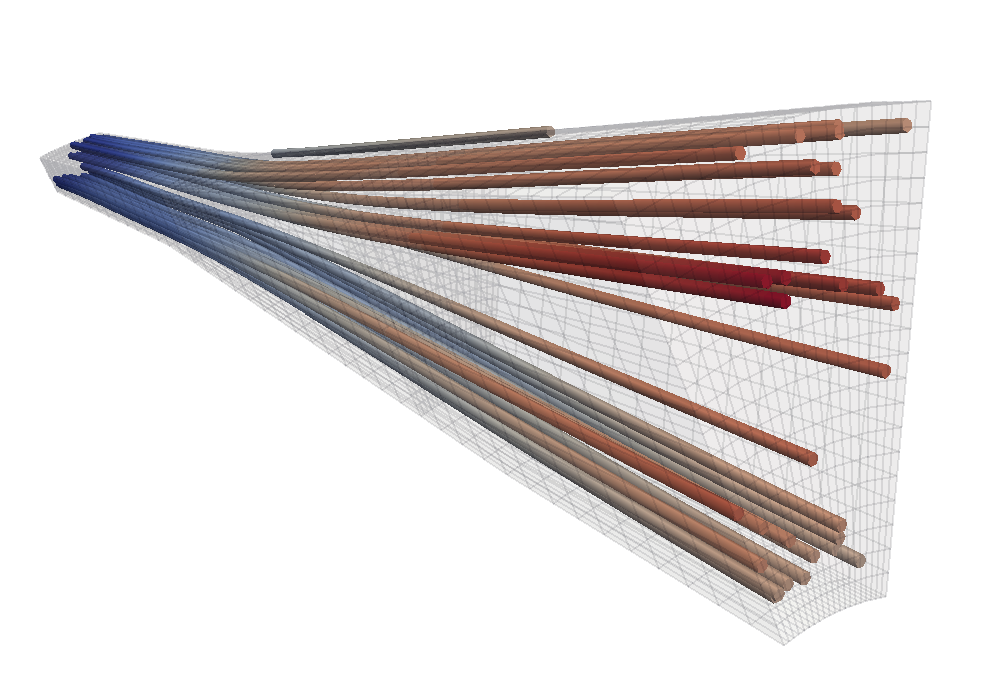
\includegraphics[width=12cm]{../3D/scramjet-1/scramjet-streamtubes.png}
\end{center}
\caption{Streamtubes passing through Katsu's scramjet combustor and nozzle.}
\label{fig:scram-tubes}
\end{figure}

\subsection{Moving Blocks}
Each block or collection of blocks visualised in ParaView can be translated, scaled 
or orientated. This may be useful when checking the operation of periodic boundary conditions, 
as illustrated in Figure \ref{fig:sc10-periodic}. A block mesh can be moved by selecting it in 
the ParaView \texttt{Pipeline Browser} panel, then selecting the \texttt{Display} tab in the \texttt{Object Inspector} 
panel and making changes to the \texttt{Transform} section of this tab.

\begin{figure}[htbp]
\begin{center}
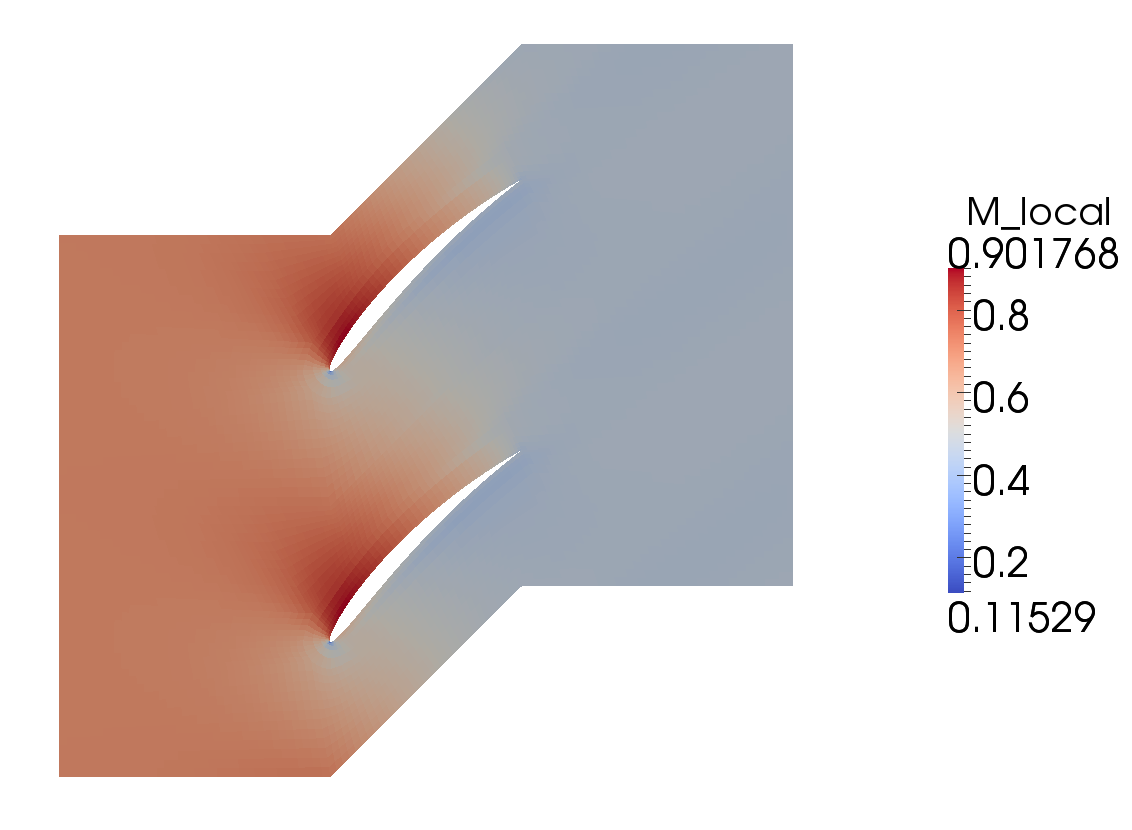
\includegraphics[width=12cm]{../2D/turbo_sc10_parametric/periodic.png}
\end{center}
\caption{Standard Configuration 10 Mach field illustrating correct operation of periodic boundary condition.}
\label{fig:sc10-periodic}
\end{figure}
